\chapter{運転行動データと可視化}\chaplab{Materials_and_Visualize}
この章では,本研究において用いられた運転行動データの詳細について述べる.またこの運転行動データから,車線変更のタイミング推定に有用であると思われる特徴を抽出した後に,車線変更直前の特徴量の変化を可視化した.
\section{運転行動データ}
本研究においては,名古屋大学が収集した運転行動データを用いた.このデータには,10名の被験者が名古屋高速道路を走行した際の,自車両の挙動や計器の情報,周辺車両との位置関係,走行中の道路の情報等の様々な運転行動が,サンプリングレート10Hzで記録されている.これらの情報のうち,本研究で利用した情報を次に示す.
\begin{itemize}
 \item 車線変更ラベル
 \item アクセルの踏み込み圧
 \item ブレーキの踏み込み圧
 \item ハンドルの操舵角
 \item 自車両中心と周辺車両中心点との相対位置
 \item 周辺車両との相対距離
\end{itemize}
\par
車線変更ラベルは,運転者が車線変更の最中であるかどうかを表しており,左車線変更に-1,直進に0,右車線変更に1の値が割り振られている.ここで,車線変更の開始のタイミングは,「車載カメラによる動画内で白線が左右に動き始めたとき」で,車線変更終了のタイミングは「その白線の動きが止まったとき」と定義されている.
\par
周辺車両との相対位置,相対速度は車載のレーザーレンジファインダーを用いて計測されており,前後方に対して最大100mの車両を検知することができる.相対位置,相対速度は,道路平面に対して車両進行方向と,その垂直方向の2次元に値を持っている.%(y軸の定義とかしちゃう?)
また,相対位置は,単に計測器から車の外縁%言葉わかんね
までの距離を出しているのではなく,自車両,周辺車両の中心位置を推定して計測している.
\par
高速道路における走行に際しては,普段通りに車線変更をして前方車両を抜かし,車両を抜かし終わったら走行車線へ戻るように被験者たちに指示が出されている.車線変更は,右車線変更左車線変更ともに,各被験者で平均30回程度行われており,すべてを合計すると,合計341回の右車線変更,335回の左車線変更が行われていた.
\section{特徴抽出}
次に,この運転行動データを用いて,車線変更のタイミングの推定に有用だと思われる特徴の抽出を行った.まず,車線変更を行う前に何らかの特徴的な操作が現れる可能性を考え,車のアクセル,ブレーキの踏み込み圧,ハンドルの操作角を特徴量として定めた.
\par
次に,周辺車両との関係性が車線変更に関わっていると考えられるため,これを特徴とする.対象とする周辺車両は,自車両に先行して走行している車両と自車両の右後方を走っている車両とする.特徴は,これらの周辺車両との相対距離,相対速度と,衝突までの時間(TTC)とした.ただし,TTCは,加速度まで考慮したうえで逆数を計算した($iTTC_{2nd}$).ここで$iTTC_{2nd}$は以下のように計算することができる.
\begin{align}
  iTTC_{2nd}=\frac{\ax}{-2\vx+\sqrt{(\vx)^2-2{\ax}x}}
  % a == 0
\end{align}

% ここに車の図を

%これは,被験者たちは,以下のように行動していたからである.はじめは前方の車両との距離が縮まったとき,右車線変更しても追い越し車線で衝突しなさそうなら右車線変更を開始する.?
%10秒に満たない時は排除くん.
\subsection{可視化}
これらの特徴量が車線変更が始まる直前にどのような変化をするのかを見るために,車線変更開始10秒前から車線変更開始0.5秒前(これを「直前」と表す)までに取った値を,0.5秒間隔でプロットした.
まず,一回の車線変更に対して上記の特徴量それぞれの組み合わせをプロットしたものが,図\ref{fig:pairplot_one_lc}である.
\begin{figure}[htbp]
  \begin{center}
    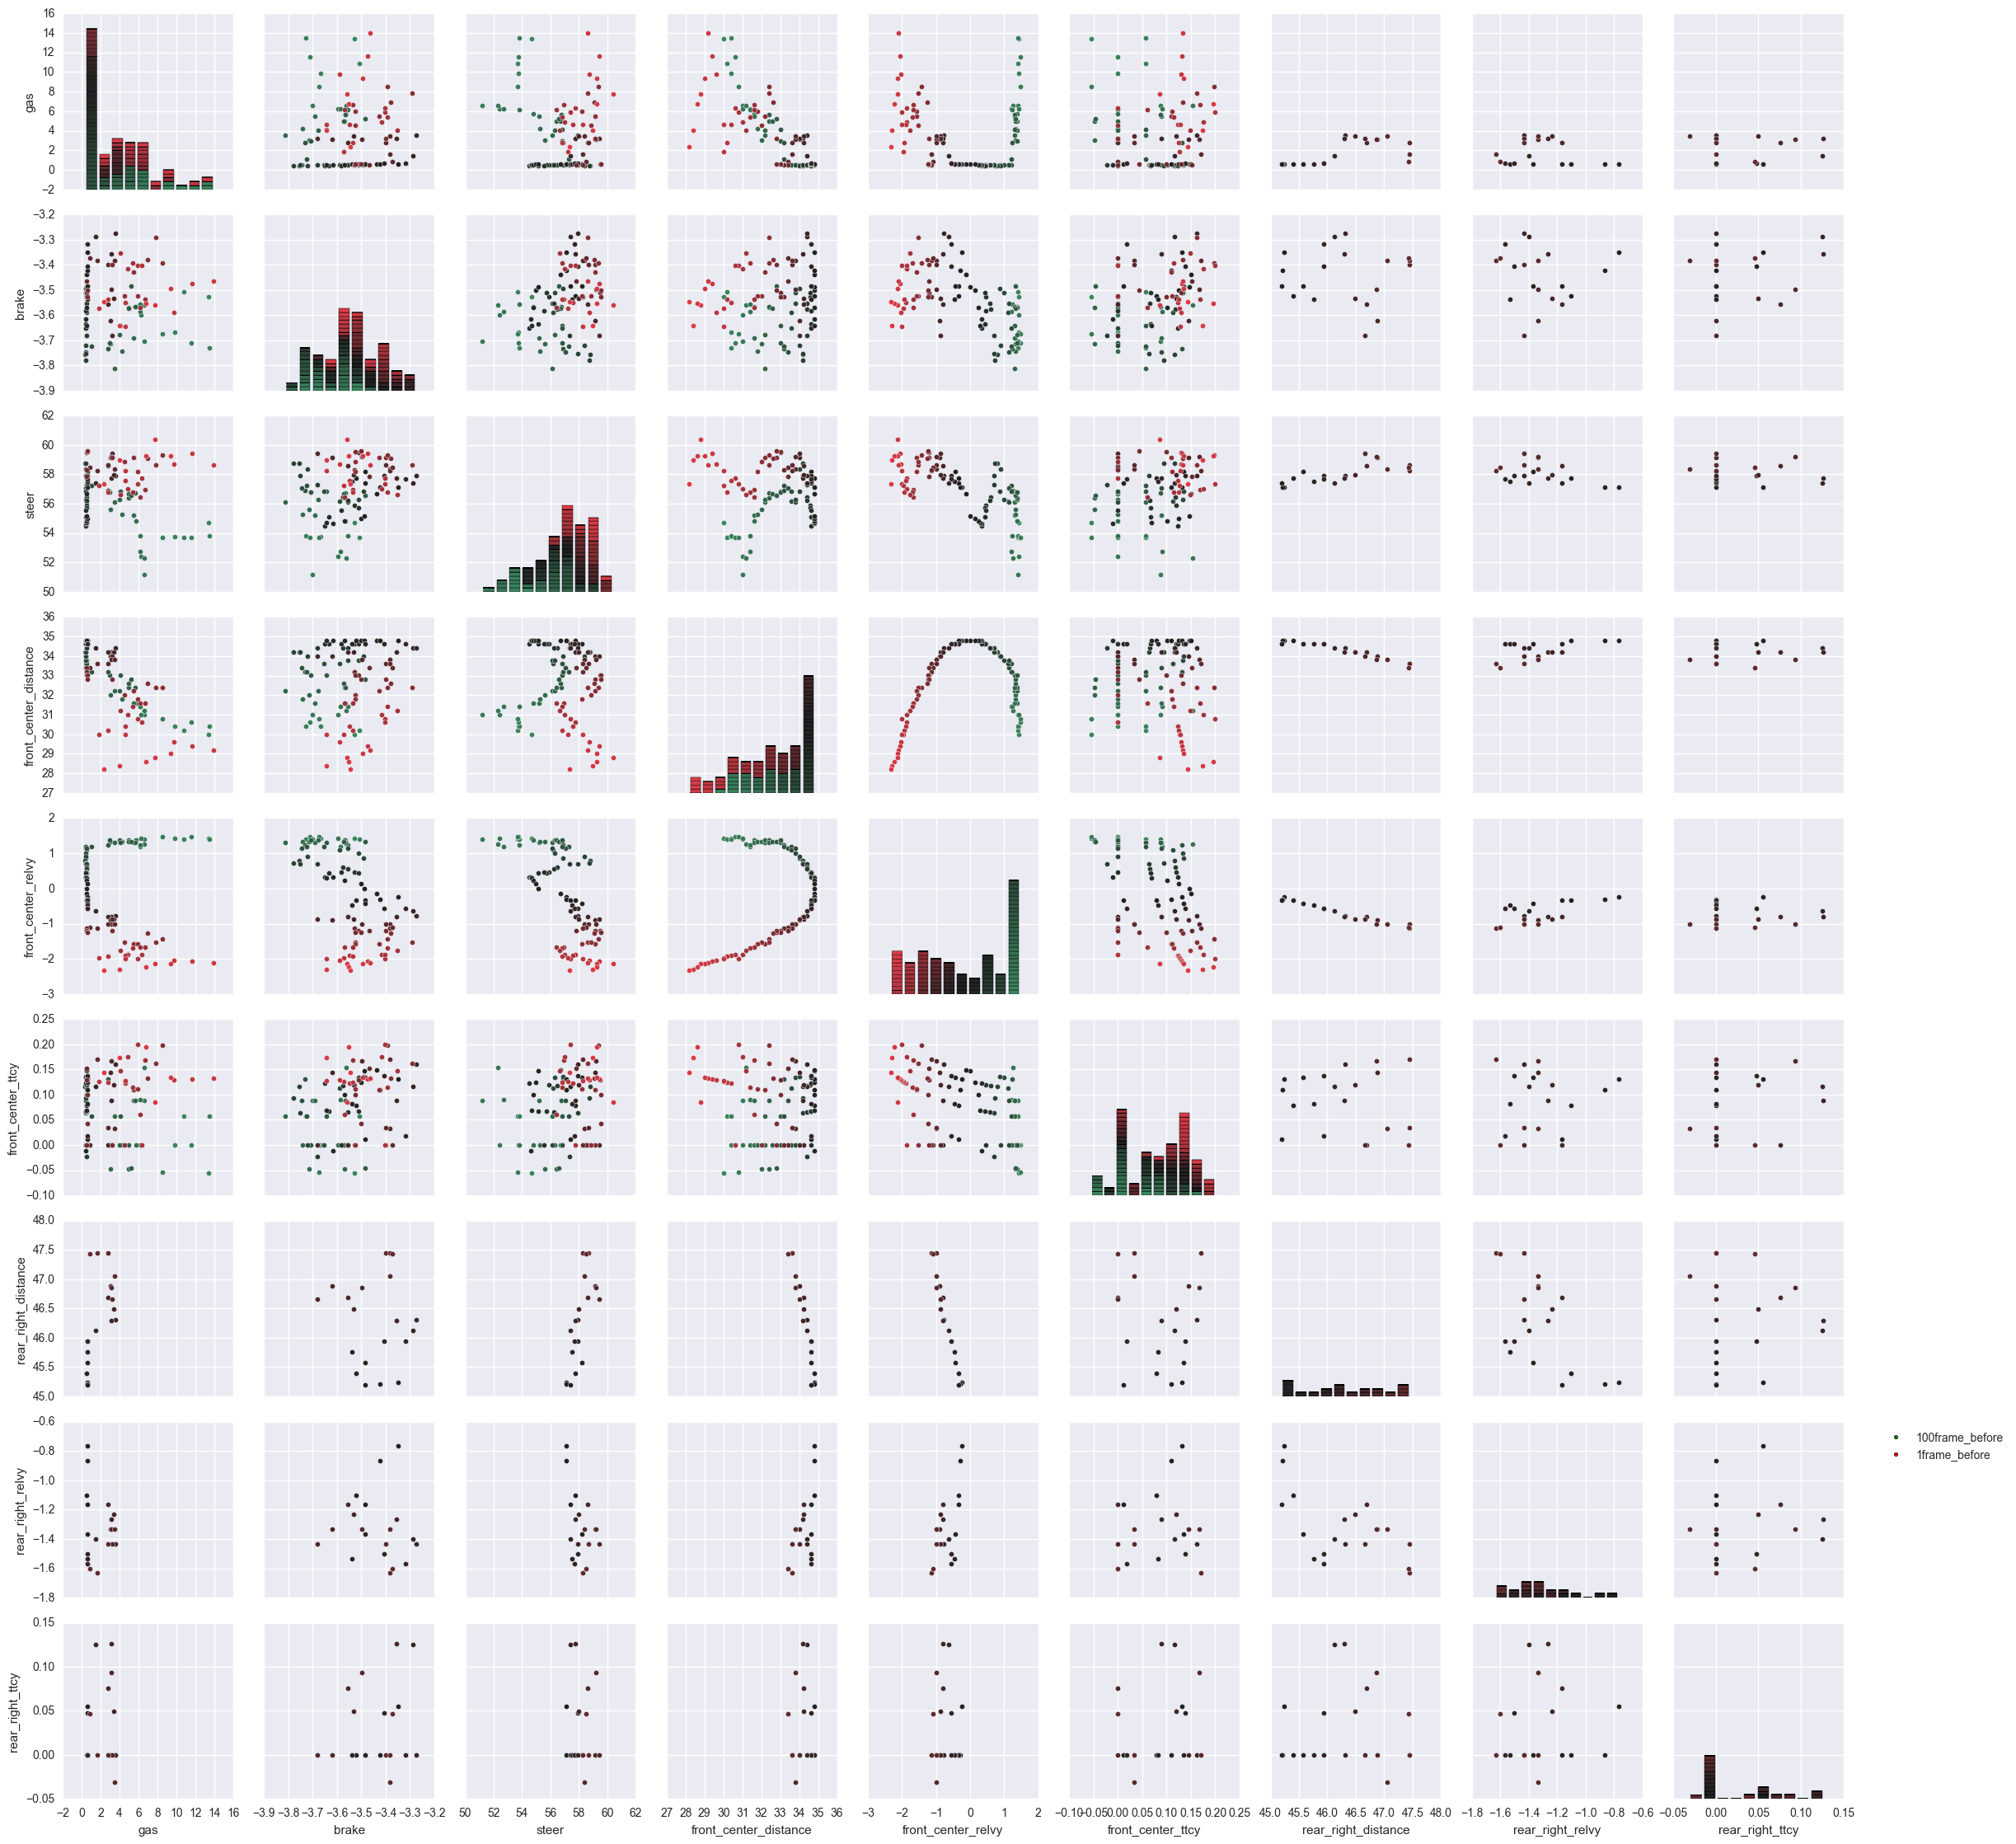
\includegraphics[clip,width=10.0cm]{fig/pairplot_one_lc.png}
    \caption{ある運転行動に対する,車線変更開始10秒前から車線変更開始までの特徴の組み合わせの散布図と,単一の特徴量のヒストグラム.上から(もしくは左から)順番に,アクセル,ブレーキ,ハンドル,前方車両との相対距離,前方車両との相対速度,前方車両との加速度考慮のTTCの逆数,右後方車両との相対距離,右後方車両との相対速度,右後方車両との加速度考慮のTTCの逆数となっている.プロットが緑から赤になるにつれて車線変更開始に近づいていることを示している.}
    \label{fig:pairplot_one_lc}
  \end{center}
\end{figure}

車線変更10秒前を緑色で,直前を赤色で,その間を黒として特徴量の変動を表している.対角の位置に当たるものがヒストグラムとなっている.ここから,どの特徴のヒストグラムを見ても色が分離されておらず,単一の特徴から車線変更か否かの分離は困難であることがわかる.しかし散布図をみてみると,先行車両との相対距離,相対速度の組み合わせにおいて時系列に沿ってデータ点が並んでおり,特徴として有用であることが伺える.
次に,先行車両との相対距離,相対速度の時系列に沿ったデータ点の移動の傾向を見るために,全時刻における,すべての車線変更トライアルについてのデータ点を表したものが\figref{scatter_ellipse}である.
\begin{figure}[htbp]
 \begin{minipage}{0.5\hsize}
  \begin{center}
    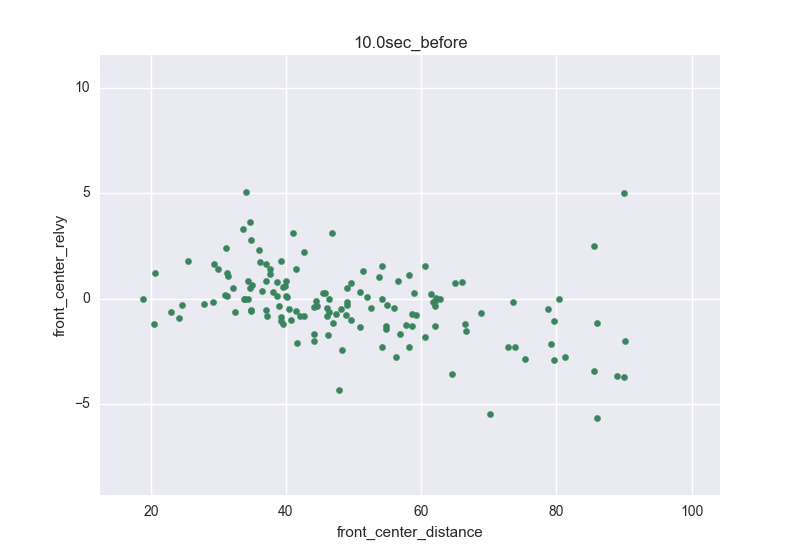
\includegraphics[width=70mm]{fig/10_sec_before.png}
  \end{center}
  \caption{車線変更開始10秒前の時点における先行車両との相対距離と相対速度を,すべてのデータにおいてプロットした散布図.x軸が距離を,y軸が速度を表す.}
  \label{fig:10_sec_before}
 \end{minipage}
 \begin{minipage}{0.5\hsize}
  \begin{center}
    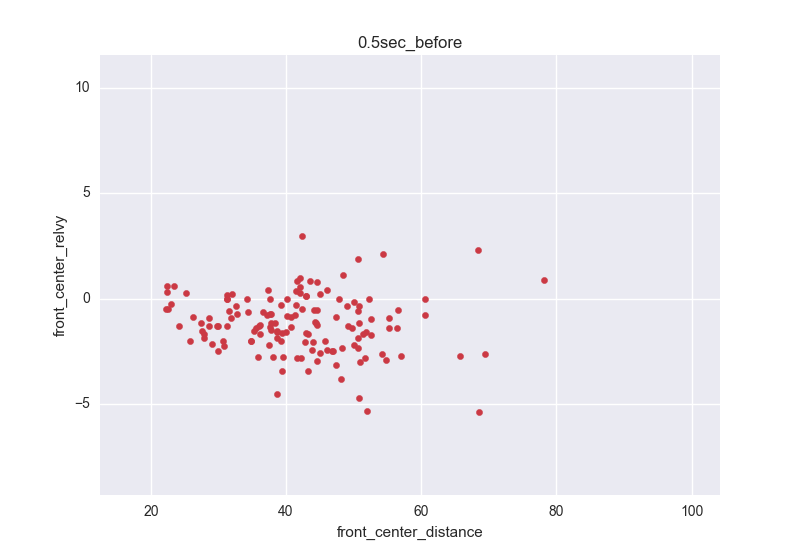
\includegraphics[width=70mm]{fig/05_sec_before.png}
  \end{center}
  \caption{車線変更開始0.5秒前の時点における先行車両との相対距離と相対速度を,すべてのデータにおいてプロットした散布図.x軸が距離を,y軸が速度を表す.}
  \label{fig:05_sec_before}
 \end{minipage}
\end{figure}

これらから,車線変更開始前の各時刻における相対距離と相対速度は,二次元の正規分布に従っていると見ることができる.また,すべての楕円をつなげたものが\figref{all_ellipse}である.
\begin{figure}[h]
  \centering
    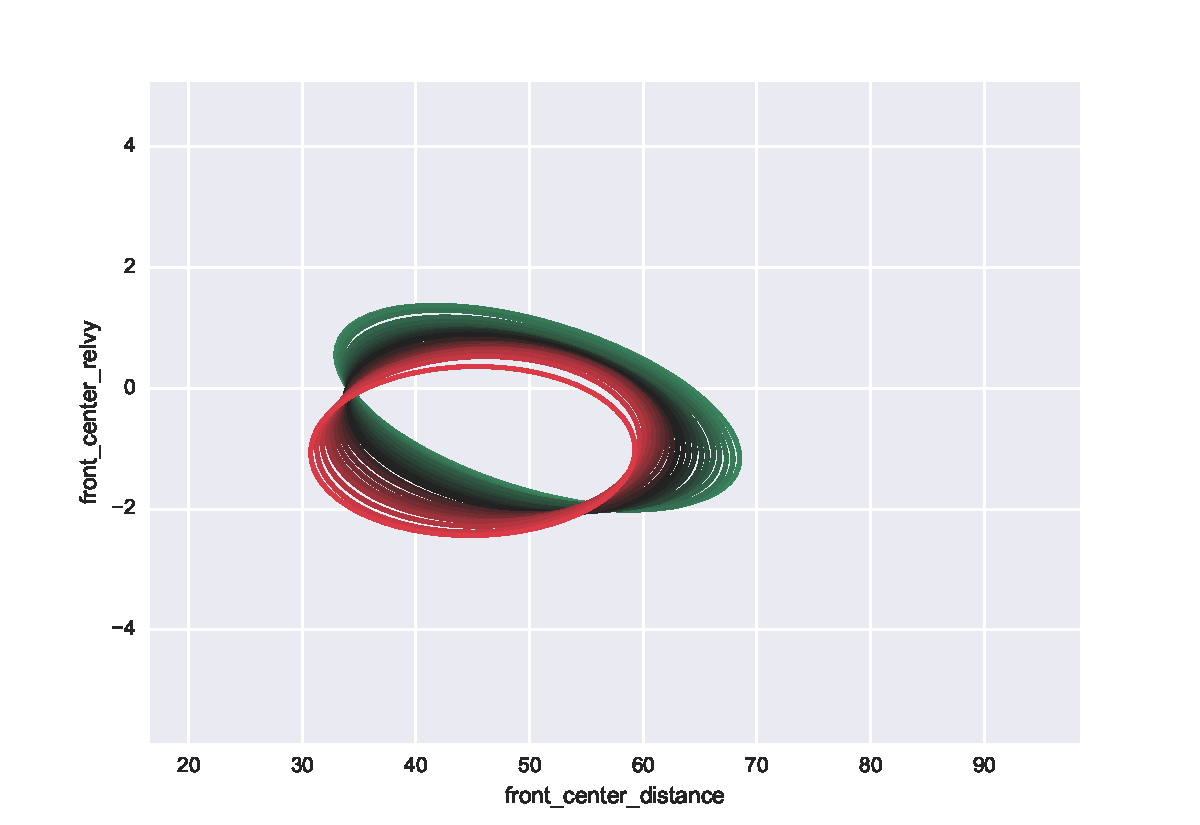
\includegraphics[width=11cm,keepaspectratio]{fig/ellipse_front_center_distance_front_center_relvy.pdf}
  \caption{\figref{scatter_ellipse}における楕円をすべて重ねたもの.}
  \label{fig:all_ellipse}
\end{figure}

各時刻の属する正規分布が収束しながら移動していっていることがわかる.
\\
また,0.5秒ごとに散布図をつなげると,データ点が回転しながら収束していくように見ることができた.この情報を特徴として持たせるために特徴量の時間差分が必要だと考え,0.5秒前のデータも特徴として盛り込み,以下に表されるような4次元の特徴とした.
\begin{align}
  \mathit{feature}_\tau=\{\dist_{\tau}^{rel},\vel_{\tau}^{rel},\dist_{\tau-1}^{rel},\vel_{\tau-1}^{rel}\}
\end{align}
ここで,$\tau$は$-20$から$-1$までの整数で,$10$秒を$0.5$秒刻みに分割した単位である.
\subsection{主成分分析}
この4次元の特徴を2次元に落とすために主成分分析(PCA)を行った.主成分分析後に得られた新たな特徴を寄与率順に$\mathbf{x}=\{\lambda_1,\lambda_2,\lambda_3,\lambda_4\}$(ただし$\lambda_3,\lambda_4$は特徴として利用せず)とおいた.
このとき,上位2成分の寄与率は以下のようになった.
\begin{table}[h]
  \centering
    \begin{tabular}{|c||c|c|c|c|} \hline
       & 第一主成分$\lambda_1$ & 第二主成分$\lambda_2$ & 第三主成分$\lambda_3$ & 第四主成分$\lambda_4$ \\ \hline
      寄与率 & 0.69 & 0.3 & 0.003 & 1.6e-05 \\ \hline
    \end{tabular}
  \caption{主成分分析により得られた特徴の寄与率.寄与率の高い順にソートしている.}
  \label{tab:pca_ratio}
\end{table}

二つの成分で,99\%超の成分を説明できることがわかる.また,PCAの主成分は,以下のようになる.
\begin{table}[h]
  \centering
    \begin{tabular}{|c||c|c|c|c|} \hline
       & 第一主成分$\lambda_1$ & 第二主成分$\lambda_2$ & 第三主成分$\lambda_3$ & 第四主成分$\lambda_4$ \\ \hline
      $\dist_{\tau}^{rel}$ & 0.66 & 0.27 & 0.00031 & 0.7 \\ \hline
      $\vel_{\tau}^{rel}$ & -0.25 & 0.66 & -0.71 & -0.019 \\ \hline
      $\dist_{\tau-1}^{rel}$ & 0.67 & 0.22 & -0.0088 & -0.71 \\ \hline
      $\vel_{\tau-1}^{rel}$ & -0.24 & 0.67 & 0.71 & -0.028 \\ \hline
    \end{tabular}
  \caption{主成分分析により得られた主成分の方向.}
  \label{tab:pca_components}
\end{table}

また,PCAを行ったあとのデータ点から得られる正規分布の時間変化を楕円で表示したものを図\ref{fig:pca_gauss}に示す.
\begin{figure}[htbp]
  \centering
    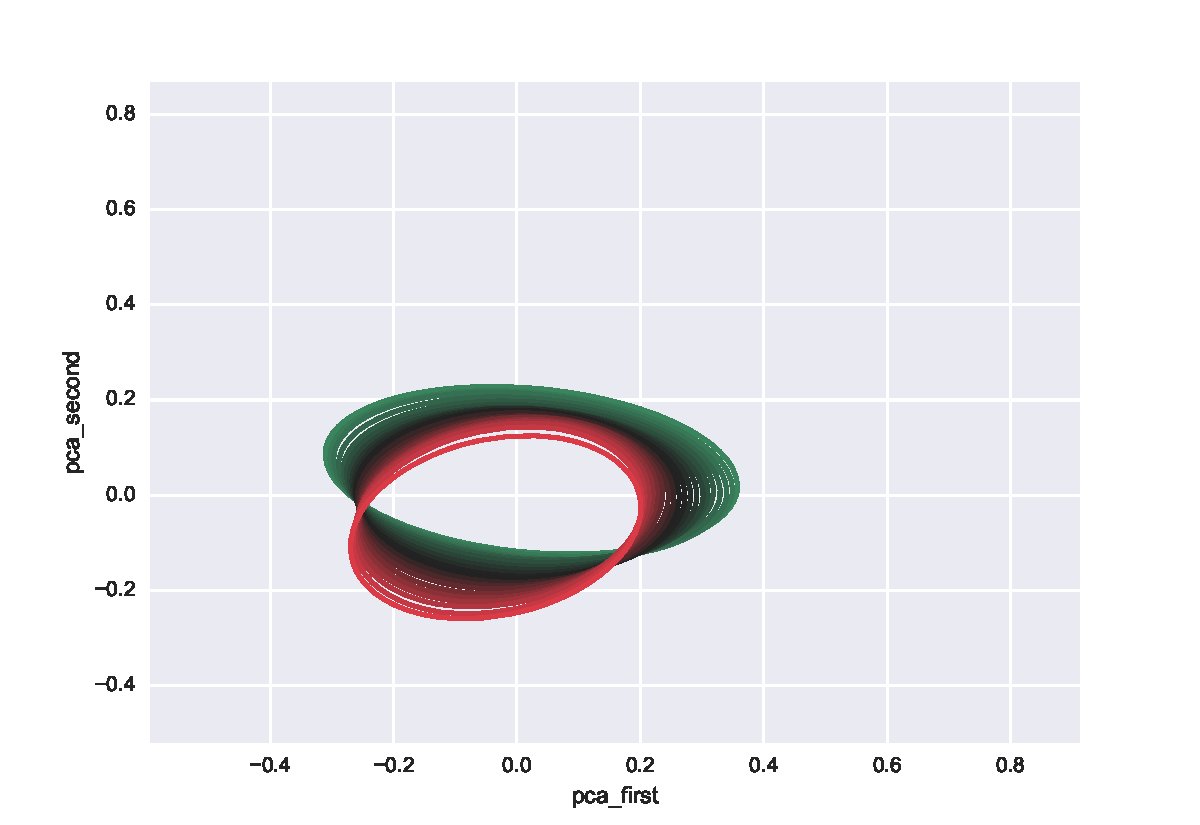
\includegraphics[clip,width=11.0cm]{fig/ellipse_pca_first_pca_second.pdf}
    \caption{主成分分析を行ったあとのデータ点から,各時刻ごとに二次元正規分布を求め,楕円としてプロットしたもの.楕円の大きさは,標準偏差の1倍になっている.緑から赤に近づくに連れて車線変更開始が近づいている.}
    \label{fig:pca_gauss}
\end{figure}

この図から,完全に車線変更開始前とそれ以外を分離することは難しいことが読み取れる.しかし,車線変更開始に近づくにつれて,楕円の平均がずれていき,分散が小さくなっていっていることから,確率的に時刻を導出できそうということがわかる.そのため,各時刻に対する正規分布を予め保持しておくことで逐次的に車線変更までのタイミングの確率分布を更新する手法が有効であると考えられる.この逐次的ベイス推定のアプローチは,細胞分裂の時刻予測についての応用\cite{Kozawa}があり,車線変更予測にも有効性が期待できる.
% 楕円の導出とか...いらんか?
% 0.5secにした理由?実用上?
